\documentclass[fleqn]{article}
\usepackage[nodisplayskipstretch]{setspace}
\usepackage{amsmath, nccmath}
\usepackage{amssymb}
\usepackage{enumitem}
\usepackage{etoolbox}
\usepackage{graphicx}
\usepackage{float}
\usepackage{changepage}
\usepackage{environ,capt-of}

\newcommand{\zerodisplayskip}{
	\setlength{\abovedisplayskip}{0pt}%
	\setlength{\belowdisplayskip}{0pt}%
	\setlength{\abovedisplayshortskip}{0pt}%
	\setlength{\belowdisplayshortskip}{0pt}%
	\setlength{\mathindent}{0pt}}
	
\title{Selection of $h_c[n]$}
\author{Owen Sowatzke}
\date{November 21, 2023}

\begin{document}

	\offinterlineskip
	\setlength{\lineskip}{12pt}
	\setlength{\parindent}{0pt} 
	\zerodisplayskip
	\maketitle
	
	The output of the inverse DFT, \texttt{h}, is one period of the Discrete Fourier Series. The causal, symmetric impulse response will be the Discrete Fourier Series from $n=-\frac{N}{2}$ to $n=\frac{N}{2}$ with the samples at $n=-\frac{N}{2}$ and $n=\frac{N}{2}$ halved. Note that halving the endpoints is necessary if we want to prevent magnitude distortion of \texttt{H(k)}.
			 
	Consider circular shifting the array of samples, \texttt{h}, by $N/2$. The circular shift should not distort the magnitude of the DFT samples.
			
	\begin{equation*}
		h_s[n] = h[(n - N/2)\ \text{mod}\ N] \leftrightarrow H[k]e^{\frac{-j{2\pi}(N/2)k}{N}}
	\end{equation*}
			
	If we take a 2N-point DFT of $h_c[n]$, the frequency response samples that we want to match to $H[k]$ are:
			 
	\begin{equation*}
		H_c[2k] = \sum_{n=0}^{2N-1}{h_c[n]e^{-\frac{j2{\pi}n(2k)}{2N}}} = \sum_{n=0}^{2N-1}{h_c[n]e^{-\frac{j2{\pi}nk}{N}}}
	\end{equation*}
			
	\begin{equation*}
		= \sum_{n=0}^{N-1}{h_c[n]e^{\frac{-j2{\pi}nk}{N}}} + \sum_{n=N}^{2N-1}{h_c[n]e^{\frac{-j2{\pi}nk}{N}}}
	\end{equation*}
			
	\begin{equation*}
		= \sum_{n=0}^{N-1}{h_c[n]e^{\frac{-j2{\pi}nk}{N}}} + \sum_{n=0}^{N-1}{h_c[n+N]e^{-\frac{j2{\pi}(n+N)k}{N}}}
	\end{equation*}
			
	\begin{equation*}
		= \sum_{n=0}^{N-1}{h_c[n]e^{-\frac{j2{\pi}nk}{N}}} + \sum_{n=0}^{N-1}{h_c[n+N]e^{-\frac{j2{\pi}nk}{N}}}
	\end{equation*}
			
	\begin{equation*}
		= \sum_{n=0}^{N-1}{(h_c[n] + h_c[n+N])e^{\frac{-j2{\pi}nk}{N}}}
	\end{equation*}
			
	Compare this to the N-point DFT of $h_s[n]$:
			
	\begin{equation*}
		H_s[k] = \sum_{n=0}^{N-1}{h_s[n]e^{\frac{-j2{\pi}nk}{N}}}
	\end{equation*}
			
	We can preserve the $H_s[k]$ samples (or the magnitude of the $H[k]$ samples) if we set:
			
	$h_c[n] + h_c[n+N] = h_s[k]$
			
	One way to do this which provides a causal filter is to let
			
	\begin{equation*}
		h_c[n] = \begin{cases}
			h_s[0]/2 & n = 0\\
			h_s[n]   & 0 < n < N\\
			h_s[0]/2 & n = N\\
			0		 & \text{otherwise}
		\end{cases}
	\end{equation*}
			
	The impulse response, $h_c[n]$, created according to the above formula is shown below:
			
	\begin{figure}[H]
		\centerline{\fbox{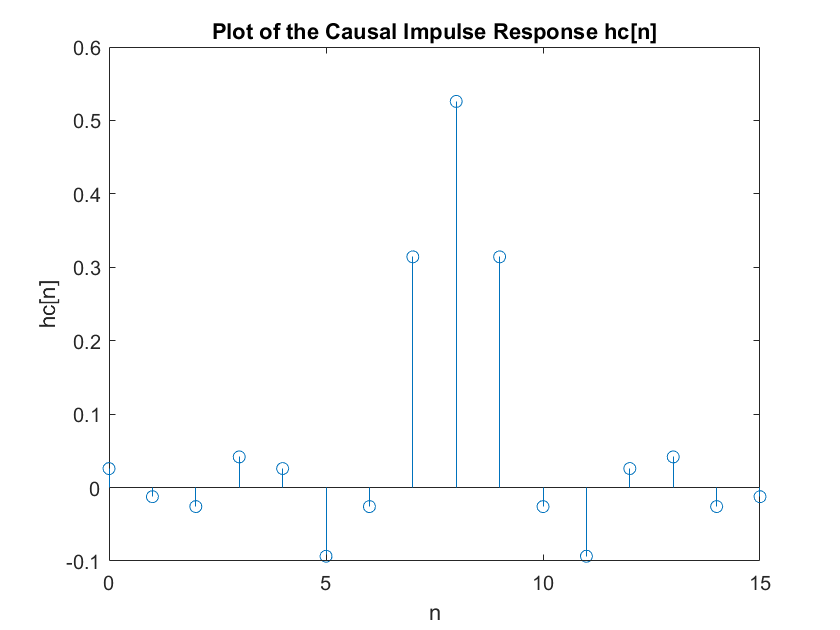
\includegraphics[width=0.5\textwidth]{prob1d_causal_impulse_response.png}}}
		\caption{Causal Impulse Response $hc[n]$}
	\end{figure}
			
	To further emphasize our selection of the causal impulse response, $h_c[n]$, we can compare $|H[k]|$ to $|H_c(e^{j\omega})|$ when the endpoints are halved and when the endpoints are not halved.
			
	\begin{figure}[H]
		\centerline{\fbox{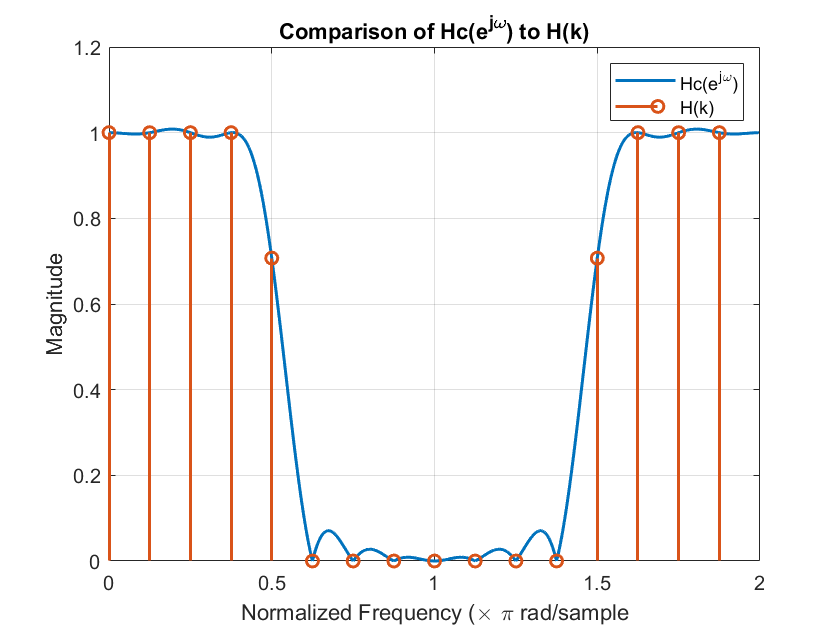
\includegraphics[width=0.5\textwidth]{prob1d_frequency_response1.png}}}
		\caption{\doublespacing Comparison of $|H(k)|$ to $|H_c(e^{j\omega})|$ when Endpoints are Halved.}
		\label{freq_response_halved_endpoints}
	\end{figure}
			
	\begin{figure}[H]
		\centerline{\fbox{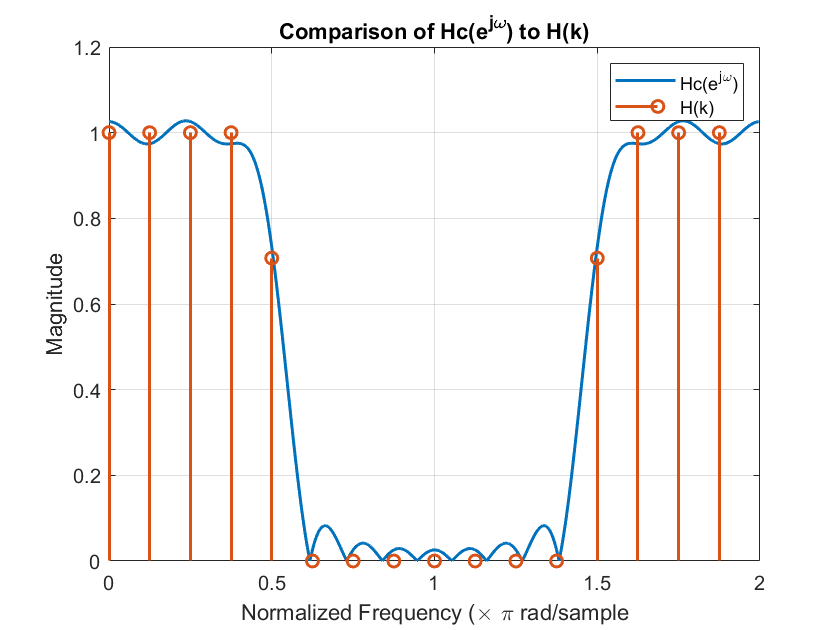
\includegraphics[width=0.5\textwidth]{prob1d_frequency_response2.png}}}
		\caption{\doublespacing Comparison of $|H(k)|$ to $|H_c(e^{j\omega})|$ when Endpoints are Not Halved.}
		\label{freq_response_raw_endpoints}
	\end{figure}
			
	Comparing, Figure \ref{freq_response_halved_endpoints} to Figure \ref{freq_response_raw_endpoints}, it is clear that halving the endpoints preserves the magnitude of the frequency response samples $H[k]$, while selecting the raw endpoints does not. Therefore, we have chosen the best option for the causal, symmetric impulse response $h_c[n]$.
\end{document}